Recently, there has been a growing need for scalable implementations of machine learning (ML)
algorithms on very large datasets (ranging from 100s of GBs to TBs of data~\footnote{This refers to
the size of the numeric features on which the algorithm operates. The raw data from which the
numeric features are extracted may be larger by 1 to 2 orders of magnitude.}). This requirement is
driven by applications such as social media analytics, web-search, computational
advertising and recommender systems.  Previous attempts at building scalable machine learning algorithms have largely been
hand-tuned implementations on specialized hardware/parallel architectures~\cite{SVMgpu}, or as noted
in~\cite{nips06}, clever methods to parallelize individual learning algorithms on a cluster of
machines~\cite{cascadesvm, paralleltutorial,parallelnmf}.  The recent popularity of MapReduce~\cite{mapreduce} as a
generic parallel programming model has invoked significant interest in implementing scalable
versions of ML algorithms on MapReduce. These algorithms have been implemented over multiple
MapReduce architectures~\cite{phoenix, scope, hadoop} ranging from multicores~\cite{nips06} to
proprietary~\cite{msrwww10,googlewww07, planet} and open source implementations~\cite{mahout}.

Much of this work reverts back to hand-tuned implementations of specific algorithms on
MapReduce~\cite{msrwww10, googlewww07}. One notable exception is~\cite{nips06} where the authors
abstract one common operation -- ``summation form'' -- and present a recipe to map instances of this
operation onto MapReduce\footnote{A class of ML algorithms compute certain global statistics which
can be expressed as a summation of local statistics over individual data points. In MapReduce, local
statistics can be computed by mappers and then aggregated by reducers to produce the global
statistics.}. Several algorithms are then expressed using multiple instances of the summation form
mapped appropriately to MapReduce jobs. This approach still leaves two fundamental problems to be
addressed:
 
\begin{itemize}
\item Each individual MapReduce job in an ML algorithm
has to be hand-coded. 
\item For better performance, the actual execution plan for the same ML algorithm has to be hand-tuned for different input and cluster sizes.
\end{itemize}

\begin{example}
\label{ex:gnmf}
The practical implications of the above two fundamental drawbacks are illustrated using this
example. Algorithm~\ref{algo:gnmf} shows a popular ML algorithm called Gaussian Non-Negative Matrix
Factorization (GNMF~\cite{LeeSeungGNMF}) that has applications in document clustering, topic modeling and computer vision. In the context
of topic modeling, V is a $d\times w$ matrix with $d$ documents and $w$ words. Each cell of V
represents the frequency of a word appearing in a document. GNMF tries to find the model of $t$
topics encoded in $W$ ($d\times t$) and $H$ ($t\times w$) matrices, such that $V\approx WH$. As seen
in the algorithm\footnote{To simplify the exposition, we leave out straightforward expressions for objective function and convergence criteria in the algorithm description.}, this is an iterative algorithm consisting of two major steps in a while loop, each step consisting of multiple matrix operations. $X^T$ denotes the transpose of a matrix $X$,
$XY$ denotes the multiplication of two matrices X and Y, $X*Y$ and $X/Y$ denote cell-wise
multiplication and division respectively (see Table~\ref{tab:notation}).
\end{example}

\begin{scriptsize}
\begin{algorithm}[h]
\caption{Gaussian Non-Negative Matrix Factorization}
\label{algo:gnmf}
\footnotesize
\begin{algorithmic}[1]
\STATE V = read(``in/V'');  //read input matrix V
\STATE W = read(``in/W'');  //read initial values of W
\STATE H = read(``in/H'');  //read initial values of H
\STATE max\_iteration $=$ 20;
%\STATE tol = 0.001; // tolerance for convergence
\STATE $i = 0$;
%\STATE $normV = norm(V)^2;$ //frobenuius norm of V
%\STATE $Obj = normV + trace( (W^T W)(H H^T)) - 2*trace(W^T X H)$
%\STATE converge = FALSE
\WHILE{i $<$ max$\_$iteration}
\STATE $H = H * (W^TV$ $/$ $W^TWH)$;  //update H
\STATE $W = W * (VH^T$ $/$ $WHH^T)$;  //update W
%\STATE //evaluate objective function and check convergence 
%\STATE $Obj =  Vfrob + trace( (W^T W)(H H^T)) - 2*trace(W^T X H)$; 
%\STATE $converge = (oldObj - Obj) < tol*oldObj$
\STATE $i = i + 1$;
\ENDWHILE
\STATE write(W,``out/W'');  //write result W
\STATE write(H,``out/H'');  //write result H
\end{algorithmic}
\end{algorithm}
\end{scriptsize}

%\begin{figure}[t]
%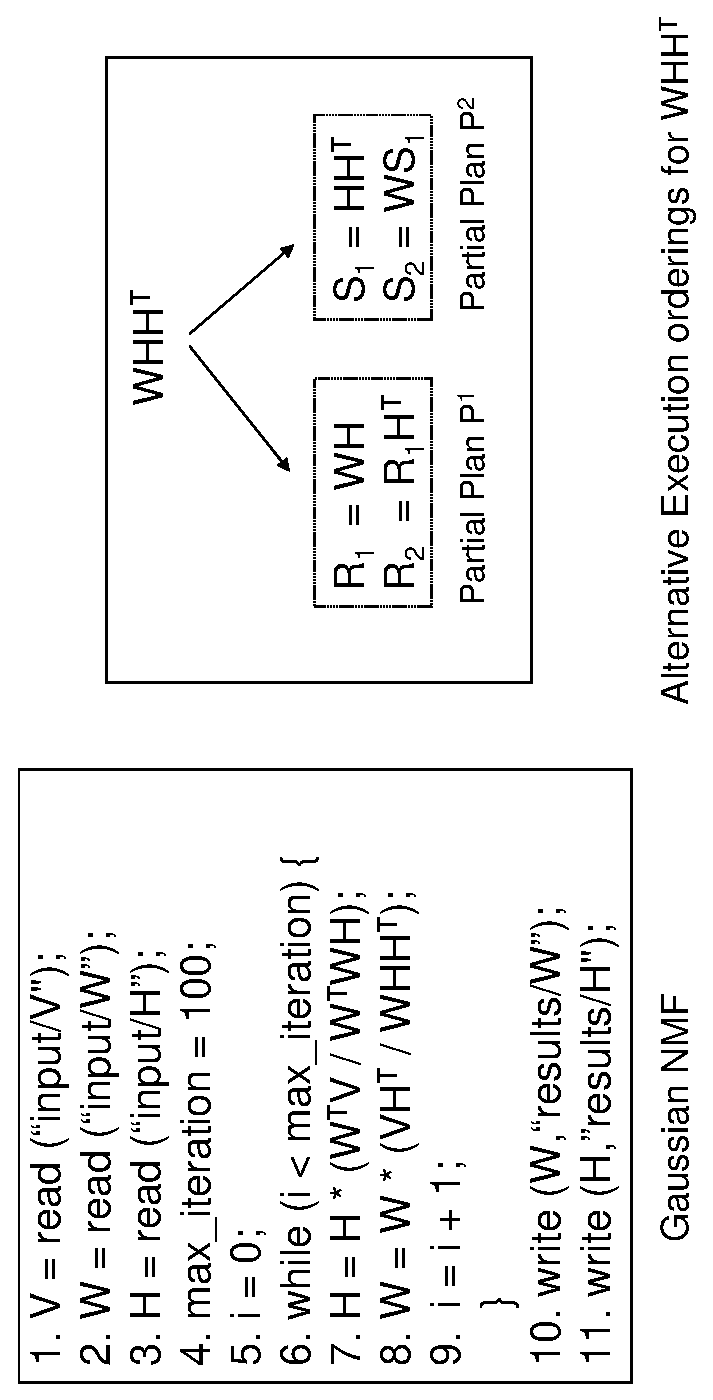
\includegraphics[angle=270,width=3.5in]{figures/gnmf.eps}
%\caption{Gaussian Non-Negative Matrix Factorization}
%\label{fig:gnmf}
%\end{figure}

Consider the expression $WHH^T$ in Step~8 of
Algorithm~\ref{algo:gnmf}. This expression can be
evaluated in one of two orders, $od1$: $(WH)H^T$ and $od2$: $W(HH^T)$. 
At first glance, picking the right order and performing this computation 
may seem straightforward, but the fact that matrix multiplication itself can be accomplished in 
multiple ways complicates matters.

Figure~\ref{fig:mmult2} and Figure~\ref{fig:mmult1} show two alternative MapReduce plans for matrix
multiplication (details of the two plans will be discussed in Section~\ref{sec:matrixmult}). The RMM
plan in Figure~\ref{fig:mmult2} implements a replication-based strategy in a single MapReduce job,
while the CPMM plan in Figure~\ref{fig:mmult1} implements a cross-product strategy that requires 2
MapReduce jobs. The choice of RMM vs CPMM is dictated by the characteristics of the matrices
involved in the multiplication. To compute $WHH^T$, we have to choose from a total of 8 plans: first
choose the order of evaluation, $od1$ or $od2$, and for the chosen order choose from RMM or CPMM for
each matrix multiplication. Instantiating the dimensionalities of the matrices reveals the need to
choose one plan over another. In the context of topic modeling, the number of topics $t$ is much
smaller than the number of documents $d$ and the number of words $w$. As a result, $od1$ will never
be selected as the evaluation order, since $WH$ produces a $d\times w$ large intermediate matrix
whereas $HH^T$ in $od2$ results in a $t\times t$ small matrix. When $d=10^7$, $w=10^5$ and $t=10$, H
is of medium size and the result of $HH^T$ is tiny. The replication based approach RMM performs very
well for both matrix multiplications. The best plan with $od2$ is to use RMM for $HH^T$ followed by
another RMM for the pre-multiplication with W.  Empirically, this plan is 1.5 times faster than the
second best plan of using CPMM followed by RMM. However, when $w$ is changed to $5\times 10^7$, size
of H increases 500 times. The overhead of replicating $H$ and $H^T$ makes RMM inferior to CPMM for
the computation of $HH^T$. On the other hand, the result of $HH^T$ remains to be a tiny matrix, so
the best plan to compute the pre-multiplication with W is still RMM. A cost model and a detailed
discussion on choosing between CPMM and RMM will be provided in Section~\ref{sec:matrixmult}.

%Note that while these optimizations are similar in spirit to join
%reordering and join method selection in relational database
%literature, applying them in the context of a declarative machine learning system on MapReduce enables unique opportunities for optimization.
%\end{example}

\customizedfig
{figures/mmult2.eps}
{RMM: Replication based Matrix Multiplication}
{fig:mmult2}
{2.6in}

\customizedfig
{figures/mmult1.eps}
{CPMM: Cross Product based Matrix Multiplication}
{fig:mmult1}
{2.4in}

As shown above, the choice of a good execution strategy depends 
significantly on data characteristics. 
Pushing this burden on programmers will have serious
implications in terms of scaling both development and execution time. 
This paper takes a step towards addressing this problem. 

\noindent {\bf Problem Statement}: Build a scalable declarative machine
learning system that
\begin{itemize}
\item exposes a declarative higher-level language for writing ML algorithms, thereby 
freeing the user from low-level implementation details and performance-tuning tasks. 
\item provides performance that scales to very large datasets and is comparable to hand-tuned implementations of individual algorithms.
\item covers a large class of ML and statistical algorithms whose computational cores are linear algebra primitives and iterative numerical optimization procedures. These include (but are not restricted to) linear statistical models, PCA, PageRank, Matrix Factorizations, and so on. 
\end{itemize}
 
The remainder of the paper is organized as follows. In Section~\ref{sec:overview}, we
present \systemml, in which ML algorithms are expressed in a higher-level language subsequently compiled and automatically parallelized to execute in Hadoop, an open source implementation of MapReduce. We then
describe the individual components of SystemML in Section~\ref{sec:arch}. 
We discuss the role of cost based optimization by showing two alternative execution plans for the expensive matrix multiplication operation.
We then present extensive experimental results
(Section~\ref{sec:experiments}) to demonstrate the scalability of \systemmltext\ and the effectiveness of the optimizations performed at various stages.

%To demonstrate the cost based optimization in SystemML, Section~\ref{sec:matrixmult} takes the expensive matrix multiplication operation as an example to discuss alternative execution plans and their associated cost models. 

%Our results demonstrate that our general-purpose system matches and at 
%times outperforms best published results based on hand-coded implementations of specific 
%algorithms.

%As background for the concepts presented in this paper, we provide a brief description of 
%MapReduce. Operationally, MapReduce consists of three phases: a \emph{Map phase} that 
%reads the data and produces a set of key-value pairs; a \emph{Shuffle phase} that sorts 
%all key-value pairs produced from the mappers by the key; and a \emph{Reduce phase} that 
%operates on all values associated with a given key and produces a new value for the same 
%key. Only the Map and Reduce phases are exposed to the user while the Shuffle phase is 
%typically internal to the platform. 
%For a more detailed description of MapReduce, the reader is referred to~\cite{mapreduce}. 
%We built our system on top of Hadoop~\cite{hadoop}, an open-source 
%implementation of MapReduce.

\begin{table*}[t]
\centering
\caption{Example operators in DML: $x_{ij}$, $y_{ij}$ and $z_{ij}$ are cells in matrices $X$, $Y$ and $Z$, respectively.} 
\label{tab:notation}
\begin{small}
\footnotesize
\begin{tabular}{|l|l|l|l|l|}
\hline
{\bf Algorithm~\ref{algo:gnmf}} & {\bf DML Statement}& {\bf Semantics} & {\bf HOP Notation} & {\bf LOP Notation}\\
\hline
$Z=X*Y$& \texttt{Z=X*Y} & cell-wise multiplication: $z_{ij}=x_{ij}*y_{ij}$ & $b(*): X, Y$ & $\grplop \rightarrow \binarylop(*)$\\
$Z=X/Y$& \texttt{Z=X/Y} & cell-wise division: $z_{ij}=x_{ij}/y_{ij}$ & $b(/): X, Y$ & $\grplop \rightarrow \binarylop(/)$\\
$Z=XY$& \texttt{Z=X\mmult Y} & matrix multiplication: $z_{ij}=\sum_{k}x_{ik}*y_{kj}$& $ab(\sum, *): X, Y$ & ($\rmmloptext$) or ($\mmcjlop \rightarrow \grplop \rightarrow \agglop(\sum)$)\\
$Z=X^T$& \texttt{Z=t(X)}& transpose: $z_{ij}=x_{ji}$ & $r(T): X$ & $\transloptext(t)$\\
& \texttt{Z=log(X)} & cell-wise logarithm: $z_{ij}=log(x_{ij})$  & $u(log): X$ & $\unarylop(log)$\\
%& \texttt{Z=X+0.5} &matrix-scalar addition: $z_{ij}=x_{ij}+0.5$ & $b(+): X, 0.5$ & $\unarylop(+)$\\
& \texttt{Z=rowSum(X)} & row-wise sums: $z_{i}=\sum_{j}x_{ij}$ & $au(\sum,\textit{row}): X$ & $\transloptext(\textit{row}) \rightarrow  \grplop \rightarrow \agglop(\sum)$\\
\hline
\end{tabular}
\BigCrunch
\end{small}
\end{table*}

